%
% JFFS3 design issues.
%
% Copyright (C), 2005, Artem B. Bityutskiy, <dedekind@infradead.org>
%
% $Id: super.tex,v 1.5 2005/11/27 14:37:50 dedekind Exp $
%

%
% THE SUPERBLOCK MANAGEMENT ALGORITHM
%
\subsection{The superblock management algorithm} \label{ref_SectionSBAlg}

To implement the superblock management scheme, JFFS3 reserves the second and
the third good eraseblocks at the beginning of the flash partition (just next
to the static eraseblock). These two eraseblocks are called \emph{anchor
eraseblocks}, or the \emph{anchor area}.

Anchor eraseblocks contain references to \emph{chain eraseblocks}. Chain
eraseblocks may either refer other chain eraseblocks or the \emph{super
eraseblock} (see figure~\ref{ref_FigureSB_01}). The number of chain eraseblocks
varies depending on the size of the JFFS3 partition. If there are $k$ chain
erase blocks, the anchor area will refer chain eraseblock 1, which will refer
chain eraseblock 2, which will refer chain eraseblock 3 and so forth. The chain
eraseblock $k$ will refer the super eraseblock.

%
% Figure with superblock management superblocks
%
\begin{figure}[h]
\begin{center}
\begin{htmlonly}
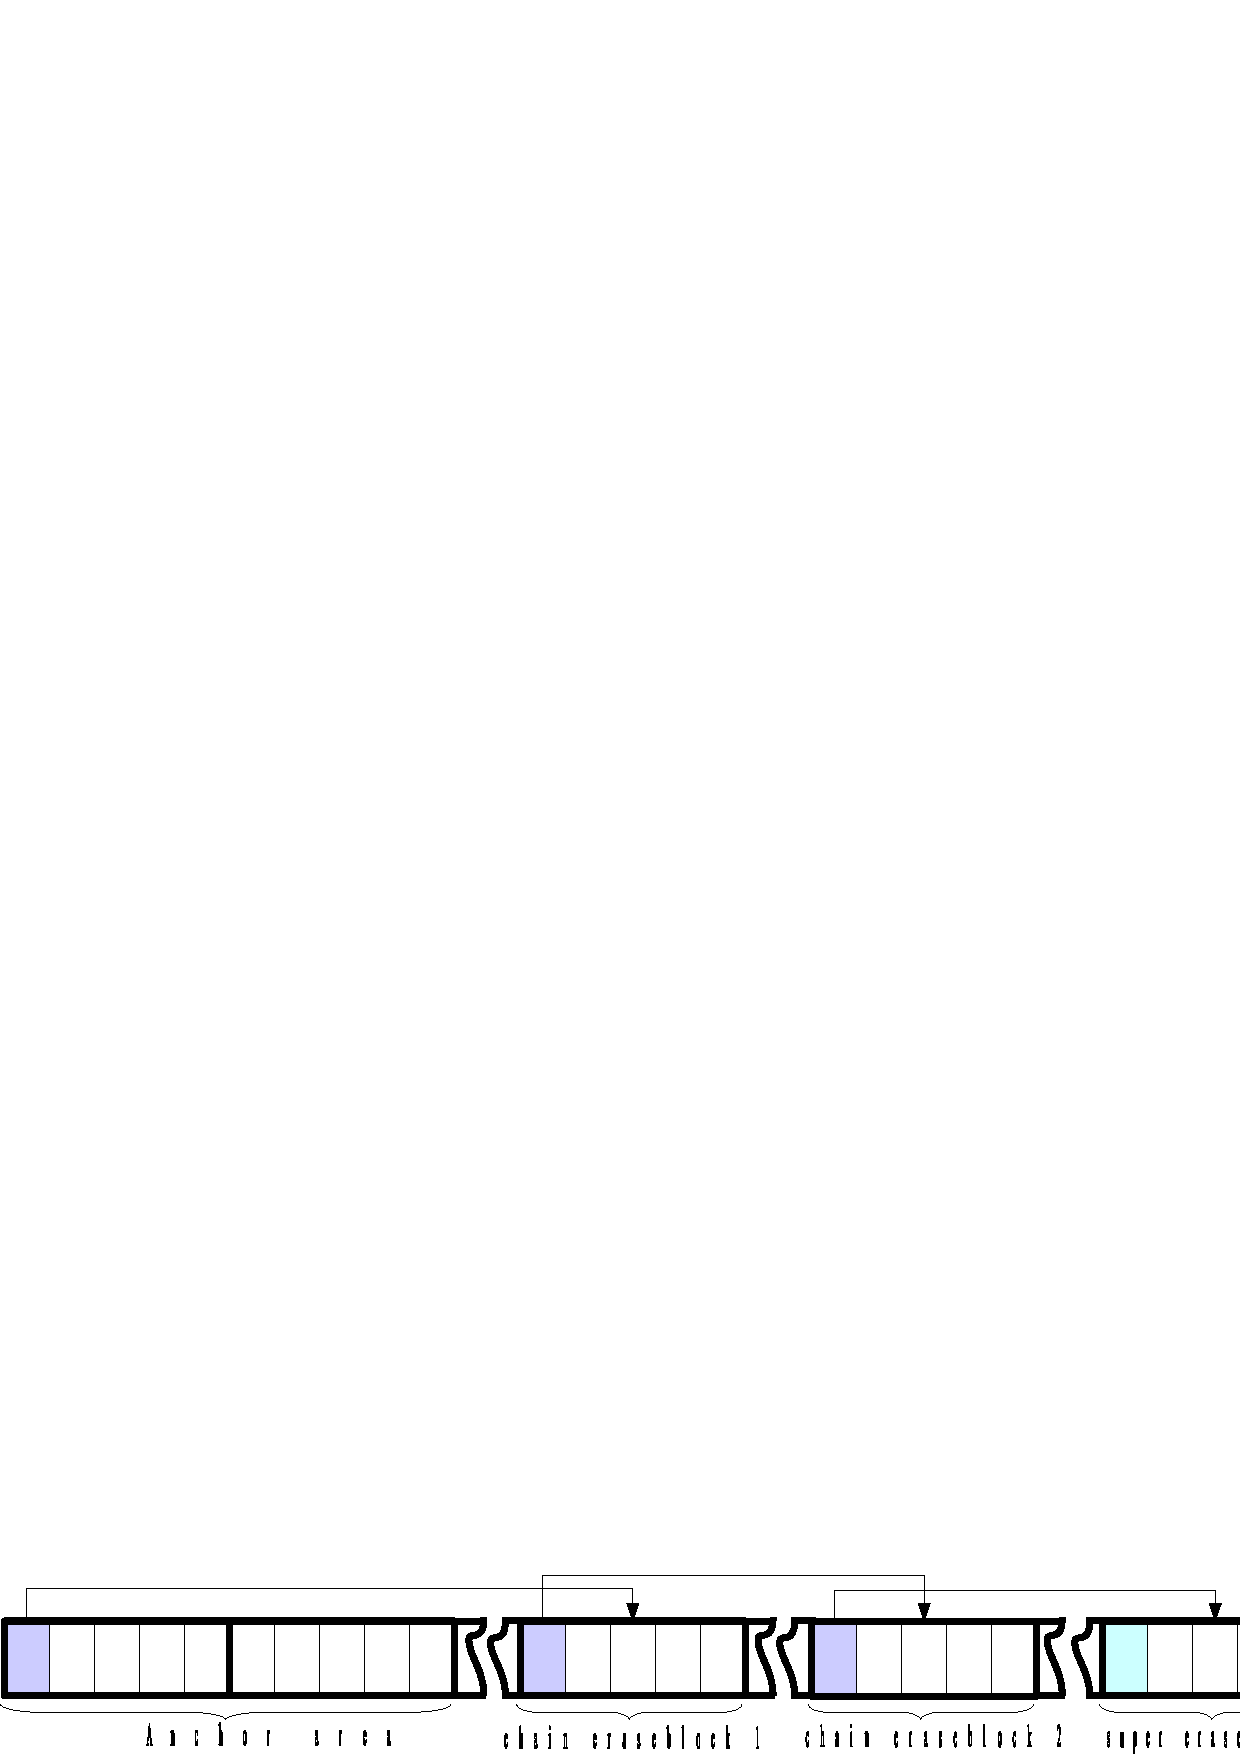
\includegraphics{pics/sb-01.png}
\end{htmlonly}
%begin{latexonly}
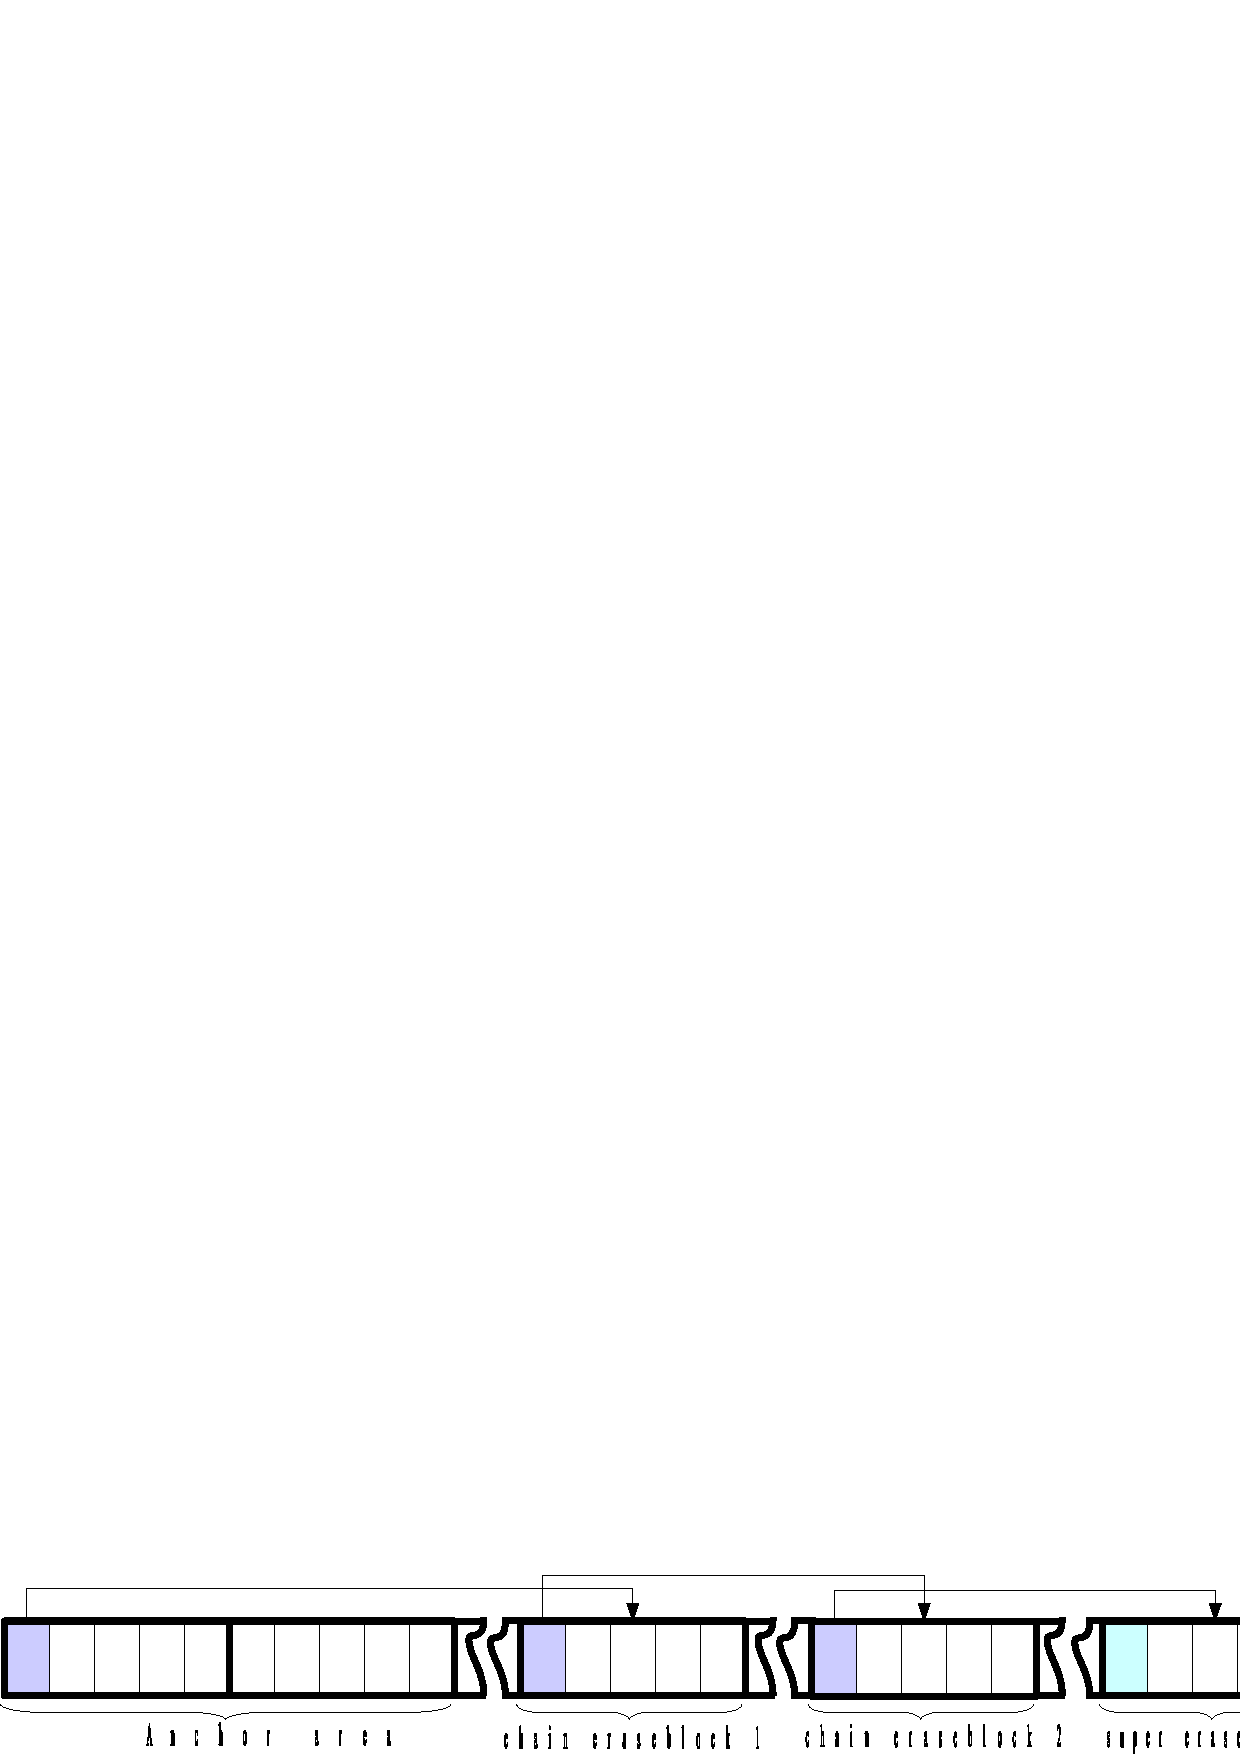
\includegraphics[width=159mm,height=21mm]{pics/sb-01.pdf}
%end{latexonly}
\end{center}
\caption{Types of eraseblocks involved to the superblock management scheme.}
\label{ref_FigureSB_01}
\end{figure}

The super eraseblock contains the superblock which takes \emph{one sector}. The
chain eraseblocks contain references to the next chain eraseblock or to the
super eraseblock.

The JFFS3 superblock management mechanisms work as follows. Suppose there are
$k$ chain eraseblocks in the current superblock management scheme. The superblock
updates are written to consecutive sectors of the super eraseblock. When
the super eraseblock has no more empty sectors, new super eraseblock is picked,
the superblock update is written to the new super eraseblock, and new reference
is written to the chain eraseblock~$k$.

Similarly, when there is no space in the chain eraseblock~$k$, new chain
eraseblock~$k$ is picked and the corresponding reference is written to chain
eraseblock~$k-1$, and so on. When there are no free sectors in the chain
eraseblock~1, new chain eraseblock~1 is picked and the corresponding
reference is written to the anchor area.

Figure~\ref{ref_FigureSB_02} presents the example of the superblock management
scheme ($k = 2$).

%
% Superblock management example
%
\begin{figure}[!t]
\begin{center}
\begin{htmlonly}
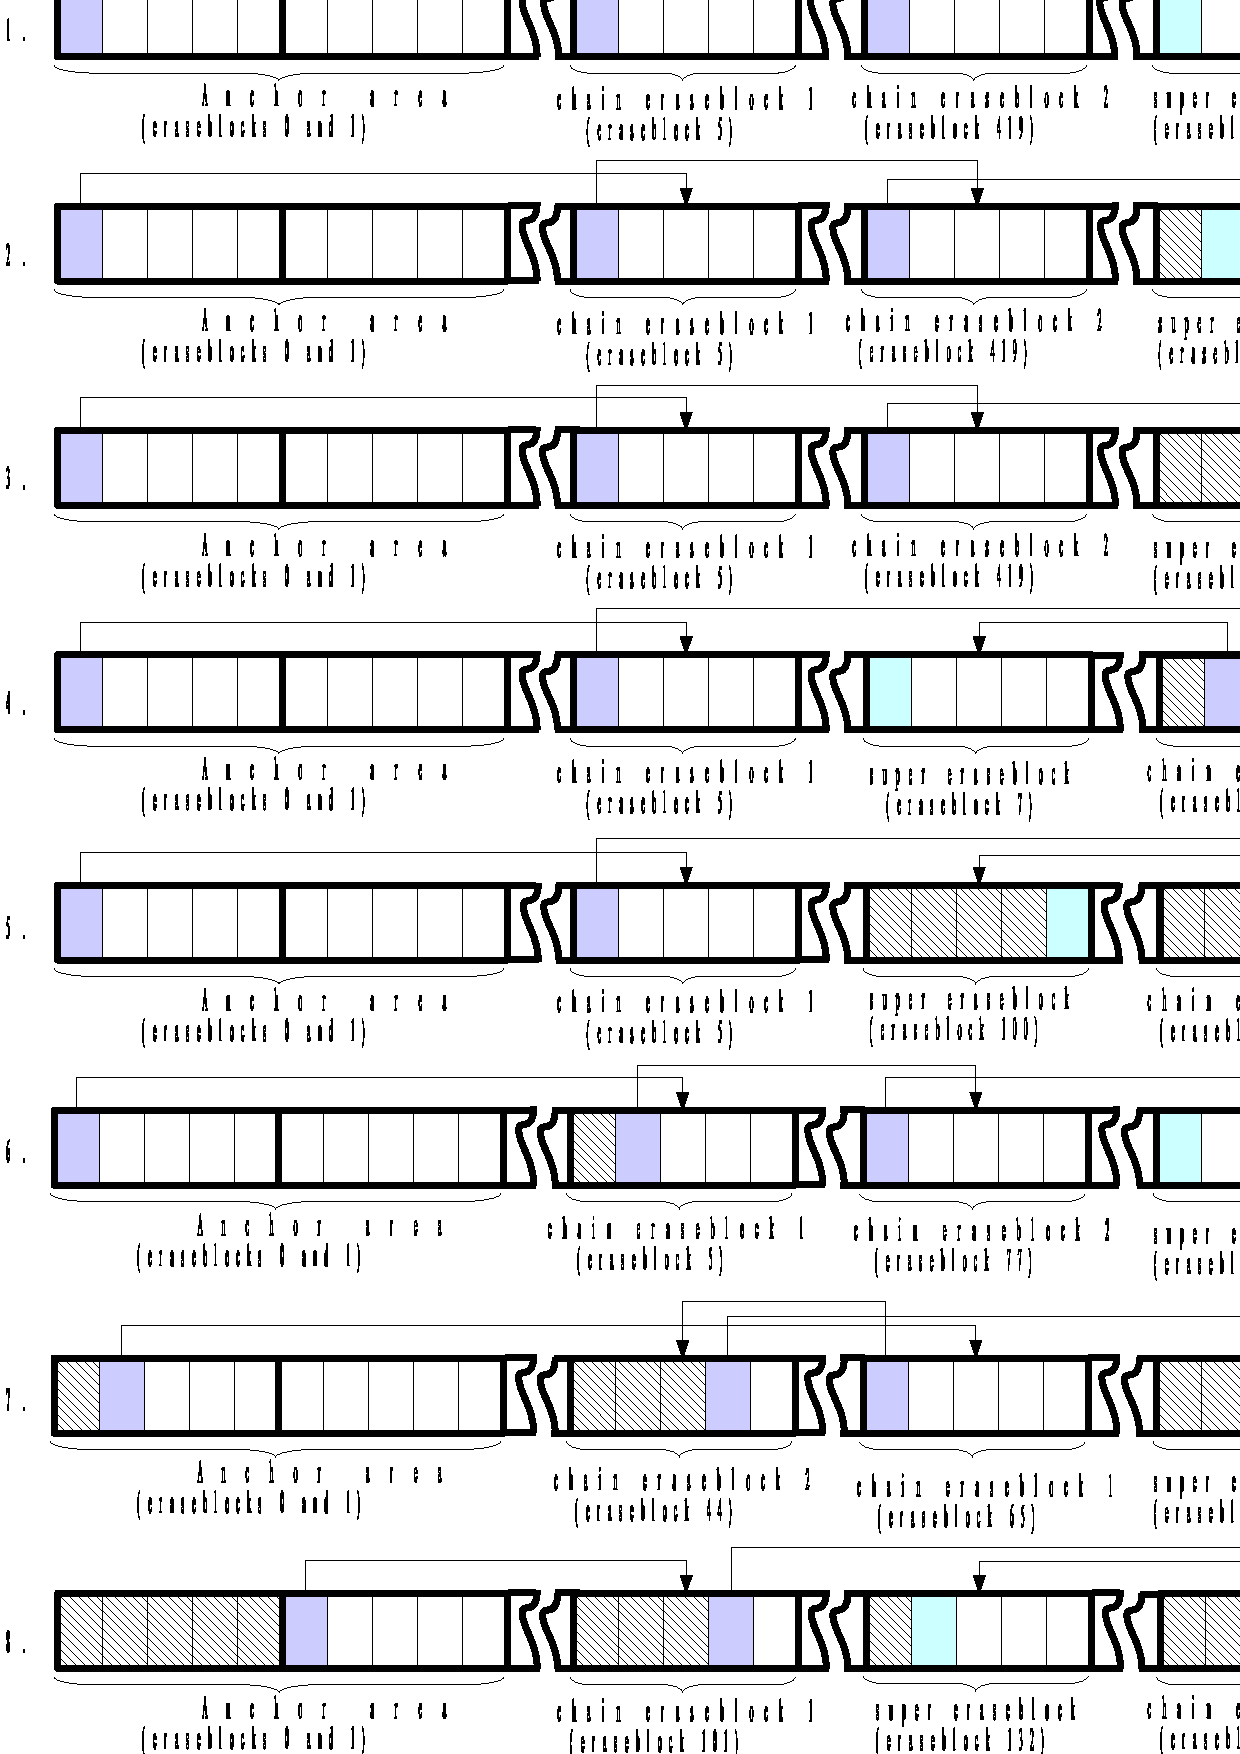
\includegraphics{pics/sb-02.png}
\end{htmlonly}
%begin{latexonly}
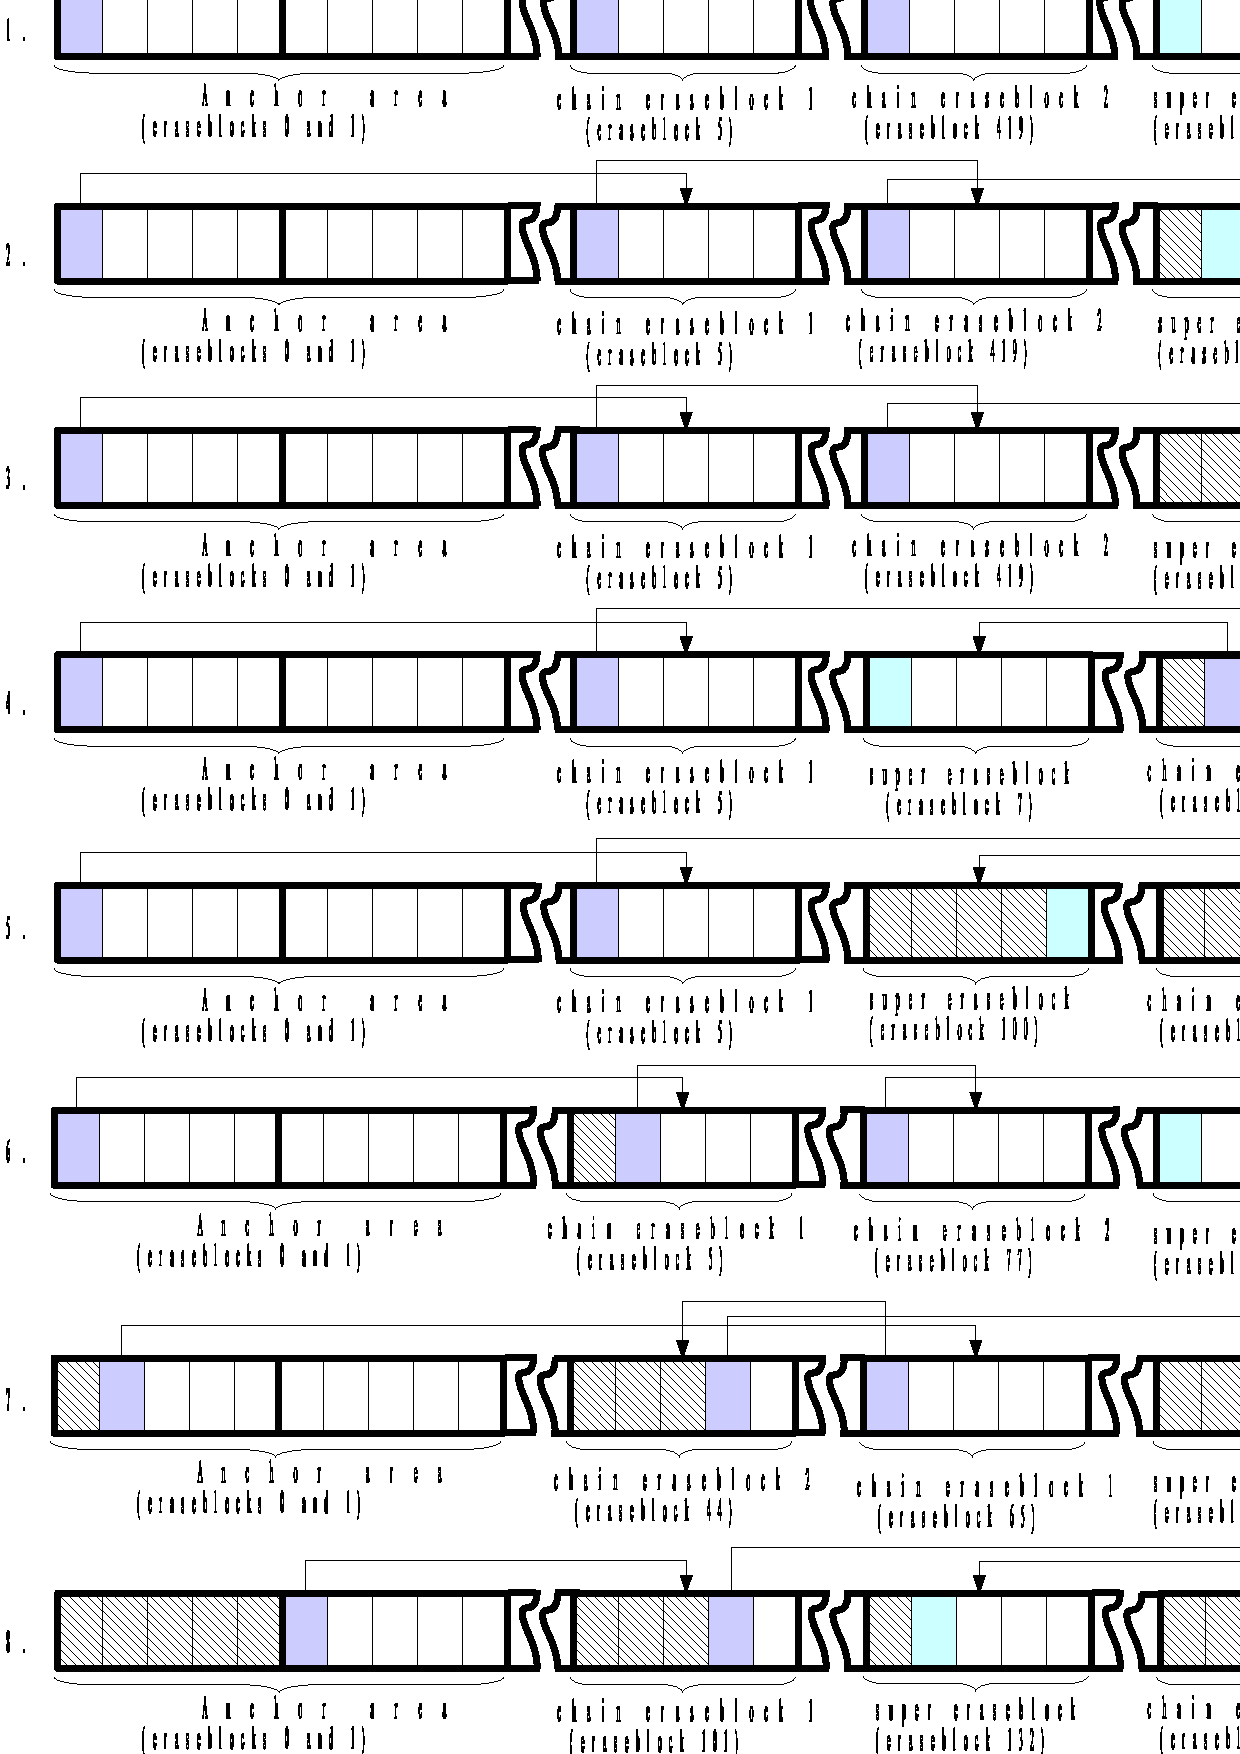
\includegraphics[width=159mm,height=200mm]{pics/sb-02.pdf}
%end{latexonly}
\end{center}
\caption{The superblock management example.}
\label{ref_FigureSB_02}
\end{figure}

\begin{enumerate}

\item Initially, there are 2 chain eraseblocks (numbers 5 and 419) and the super
eraseblock (number~501). There is a reference in the first sector of the anchor
area which refers the chain eraseblock~1. The first sector of the chain
eraseblock~1 refers the chain eraseblock~2, and the first sector of the chain
eraseblock~2 refers the super eraseblock. The first sector of the super
eraseblock contains the superblock.

\item After the superblock has been updated, the second sector of the super
eraseblock contains the valid copy of the superblock and the first sector
contains garbage.

\item The superblock has been updated many times and the valid superblock is at
the last sector of the super eraseblock while the other sectors of the super
eraseblock contain garbage.

\item As there were no free sectors at the super eraseblock, new super
eraseblock was chosen (eraseblock number~7) and the superblock update was
written to the first sector of the new super eraseblock. As the super
eraseblock changed its position, the corresponding reference at the chain
eraseblock~2 was updated. It was updated \mbox{out-of-place} and now the first
sector of the chain eraseblock~2 is dirty while the second sector contains the
valid reference to the new super eraseblock.

\item The superblock has been updated many times and the super eraseblock
changed its position many times and it is currently at the eraseblock number
100. The reference to the super eraseblock was also updated many times and at
the moment the last sector of the chain eraseblock~2 contains the valid
reference while the other sectors are obsolete. Similarly, the last sector of
the super eraseblock contains valid superblock while the other sectors are
obsolete.

\item When the next superblock update came, there were no free sectors at the
super eraseblock and new super eraseblock was picked (eraseblock number~398)
and the valid copy of the superblock is currently at the first sector of the
eraseblock number~398, Also, there were no free sectors at the chain
eraseblock~2 and new chain eraseblock~2 was picked (eraseblock number~77), so
the first sector of the eraseblock~77 contains the valid reference to the super
eraseblock. Since the chain eraseblock~2 changed its position, the
corresponding reference at the chain eraseblock~1 was updated and at the moment
the second sector of the chain eraseblock~1 contains the valid reference to the
chain eraseblock~2 while the first sector is dirty.

\item And analogously, after many superblock updates, the chain eraseblock~1
was updated many times and when it became full it changed its position. Sure,
the chain eraseblock~2 and the super eraseblock changed their positions many
times as well. So, at the moment, the chain eraseblock~1 is at the eraseblock
number~65, the chain eraseblock~2 is at the eraseblock~44 and the super
eraseblock is at the eraseblock~120. When the chain eraseblock~1 changed its
position, the corresponding reference at the anchor area was updated and
currently the second sector of the anchor eraseblock~1 contains the valid
reference to the chain eraseblock~1 while the firs sector is dirty.

\item And even more superblock updates happened. The anchor area was updated
many times. When there were no free sectors at the anchor eraseblock~1, the
anchor eraseblock~2 was used. So, at the moment, the valid reference to the
chain eraseblock~1 is at the first sector of the anchor eraseblock~2. From now
on, the first anchor eraseblock may be erased and may be used again when the
second anchor eraseblock is full.

\end{enumerate}

The following are important notes about the JFFS3 superblock management.

\begin{itemize}

\item The superblock takes one sector so the super eraseblock may be updated at
most $N$ times ($N$ is the number of sectors in the eraseblock).

\item In case of NAND flash, the sector is the real minimal physical
input/output unit, so only $N$ updates are possible in anchor eraseblocks
and in chain eraseblocks. But if the real input/output unit is smaller then
the sector (i.e., if JFFS3 works on top of NOR flash) the advantage of this may
be used and more references may be packed into one anchor or chain eraseblock.

\item When JFFS3 picks new chain/super eraseblock, the common JFFS3
\mbox{wear-levelling} scheme is utilized.

\item Anchor area has 2 eraseblocks in order to ensure the tolerance to unclean
reboots~-- one anchor eraseblock may be safely erased while the other is being
used.

\item When a new reference is written to anchor/chain eraseblocks, the previous
reference becomes dirty and on mount JFFS3 should find the valid reference. To
facilitate this, each reference has its version number. Each subsequent
reference has higher version then the previous. Hence, JFFS3 may use the
binary search algorithm to quickly find the valid reference.

\item As unclean reboot may happen anytime, no anchor/chain/super eraseblocks
are erased before the whole chain has been updated. This makes it possible to
recover from unclean reboots if they happen while the chain of the
\mbox{superblock-related} eraseblocks is being updated.

\end{itemize}

%
% THE LENGTH OF THE CHAIN
%
\subsection{The length of the chain}

The number of required eraseblocks in the superblock management scheme depends
on the size of the JFFS3 partition. The larger the partition, the more levels
are needed. This is determined by the need to ensure that the anchor area is
not worn out earlier then the rest of the JFFS3 partition.

Denote the number of required chain eraseblocks plus one (the super
eraseblock) $m$ and calculate $m$ assuming the worst case scenario: any
file system data update requires the superblock update. This would correspond
to synchronous JFFS3 operation mode with \mbox{zero-length} journal.

Obviously, what is wanted is to be sure that the anchor area is not worn out
earlier then the data area, i.e. the following inequality should be true:

\begin{equation}
\frac{T_A}{T_D} \geqslant 1,
\label{ref_EquationSBIneq}
\end{equation}
where $T_A$ is the period of time of the total anchor area wear and $T_D$ is
the period of time of the total data area wear. Note, the whole JFFS3 partition
excluding the static superblock and the anchor area is referred to as the
\emph{data area}.

If $R_A$ is the average rate of the anchor area updates (sectors per second),
$R_D$ s the average rate of the data area updates and $N$ is the number of
sectors per the eraseblock, then the anchor area will be written to with rate
$R_A/N$ eraseblocks per second and the data area will be written to with the
rate $R_D/N$ eraseblocks per second. So, JFFS3 will need to erase $R_A/N$
eraseblocks per second in the anchor area and $R_D/N$ eraseblocks per second in
the data area. Therefore, $T_A$ and $T_D$ may be expressed as

$$
T_A = \frac{2D \cdot N}{R_A},
$$
$$
T_D = \frac{(M-3) \cdot D \cdot N}{R_D},
$$
where $D$ is the maximum number of flash eraseblock erase cycles, and $M$ is
the number of non-bad eraseblock on the JFFS3 partition. We subtracted 3 from
$M$ to get the number of eraseblocks in the data area.

\begin{equation}
\frac{T_A}{T_D} = 2 \cdot \frac{R_D}{(M-3) \cdot R_A}.
\label{ref_Equation_TA_and_TD}
\end{equation}

If $m = 0$, i.e., there are no chain/super eraseblocks and the superblock is
stored in the anchor area, then taking into
account~(\ref{ref_Equation_TA_and_TD}) and that in this case $R_A = R_D = R$,
we have

$$
\frac{T_A}{T_D} = \frac{2}{(M-2)}.
$$

Suppose $m = 1$. i.e., there are no chain eraseblocks and only the super
eraseblock is used. In this case each file system data update will require (a)
the superblock update in the data area and (b) the anchor area update.
Therefore, the anchor area will be written $N$ times less frequently then when
$m = 0$ and the data area will be written $2$ times more frequently then when
$m = 0$. This means, that $R_A = R/N$ and $R_D = 2R$ and
from~(\ref{ref_Equation_TA_and_TD}) we have

$$
\frac{T_A}{T_D} = 2 \cdot \frac{2N}{M-3}.
$$

When $m = 2$, i.e. the chain eraseblock 1 and the super eraseblock are used,
the anchor area will be written $N^2$ times less frequently, while the data
area will be written $2+1/N$ times more frequently then when $m = 0$ (one
superblock update on each file system update and one chain eraseblock 1 update
per $N$ superblock updates). Therefore, $R_A=R/N^2$ and $R_D = (2 + 1/N) \cdot
R$ and from~(\ref{ref_Equation_TA_and_TD}) we have

$$
\frac{T_A}{T_D} = 2 \cdot \frac{2N^2+N}{M-3}.
$$

For $m = 3$, analogously,

$$
\frac{T_A}{T_D} = 2 \cdot \frac{2N^3 + N^2 + N}{M-3},
$$
and for $m = 0,1,2,\ldots$

$$
\frac{T_A}{T_D} = 2 \cdot \frac{2N^m + N^{m-1} + \ldots + N}{M-3}.
\label{ref_Equation_TA_div_TD}
$$

Consequently, from~(\ref{ref_EquationSBIneq}) we have the following inequality:

$$
2 \cdot \frac{2N^m + N^{m-1} + \ldots + N}{M-3} \geqslant 1,
$$
or neglecting the minor components,

$$
\frac{4N^m}{M-3} \geqslant 1,
$$
or

\begin{equation}
m \geqslant log_N{\frac{M-3}{4}}.
\label{ref_EquationSBIneq1}
\end{equation}

Thus, form~(\ref{ref_EquationSBIneq1}) it is obvious that the JFFS3 superblock
management scheme scales logarithmically.

Table~\ref{ref_TableNANDLevels} shows the value of $m$ for different types of
existing NAND flashes (see~[\ref{ref_TOSHIBA_TC58DVM92A1FT}],
[\ref{ref_TOSHIBA_TH58NVG1S3AFT05}], [\ref{ref_STMICRO_NAND08GB}],
and~[\ref{ref_SMSUNG_K9K1G08X0B}]).

\begin{table}[h]
\begin{center}
\begin{tabular}{llllll}
\textbf{Type} & \textbf{Size} & \textbf{Sect. size} & $\bf M$ & $\bf N$ &
\textbf{$\bf m$}\\
\hline
Toshiba TC58DVM92A1FT   & 64MB  & 16KB  & 4096  & 32 & 2\\
Toshiba TH58NVG1S3AFT05 & 512MB & 128KB & 4096  & 64 & 2\\
ST Micro NAND08G-B      & 1GB   & 128KB & 8192  & 64 & 2\\
Samsung K9K1G08X0B      & 2GB   & 128KB & 16384 & 64 & 2\\
\end{tabular}
\caption{The length of the JFFS3 superblock management chain for different
types of existing NAND flashes.}
\label{ref_TableNANDLevels}
\end{center}
\end{table}

Note, providing that $N=64$, $m=3$ is enough to guarantee acceptable anchor
area wear leveling for up to 128GB flash, $m=4$~-- for up to 8TB flash (the
inequality~\ref{ref_EquationSBIneq1}).

%
% THE SUPERBLOCK SEARCH
%
\subsection{The superblock search}

To find the superblock during mount, JFFS3 finds the valid reference in the
anchor eraseblocks, then finds the valid reference in chain erase blocks
$1$,~$2$,~$\ldots$,~$m-1$, and finally finds the valid superblock in the super
eraseblock. Since JFFS3 assigns versions to records in anchor/chain/super
eraseblocks and the versions are increased by one on every update, the binary
search algorithm may be used to quickly find the valid sector.

The valid reference in the anchor area may be found after $log_2(2N)+2$ steps
(one step involves one sector read operation), the reference in chain/super
eraseblocks~-- after $log_2(N)+2$ steps. Thus, to find the superblock, JFFS3
must read

$$
S = 2m + log_2(2N) + (m - 1) \cdot log_2(N)
$$
sectors.

Table~\ref{ref_TableNANDTimes} contains the approximate superblock search time
for different existing NAND flashes
\footnote{the calculated superblock search time does not contain the ECC/CRC
checking overhead as well as any other CPU overhead.}.

\begin{table}[h]
\begin{center}
\begin{tabular}{lllllll}
\textbf{Type} & \textbf{Size} & $\bf N$ & $\bf m$ & \textbf{Sect. read} & $\bf
S$ & \textbf{SB find}\\
\hline
Toshiba TC58DVM92A1FT & 64MB & 32 & 2 & $\sim$50$\mu$s  & 22 & $\sim$1.1ms\\
ST Micro NAND08G-B    & 1GB  & 64 & 2 & $\sim$130$\mu$s & 25 & $\sim$3.3ms\\
Samsung K9K1G08X0B    & 2GB  & 64 & 2 & $\sim$70$\mu$s  & 25 & $\sim$1.6ms\\
\end{tabular}
\caption{The superblock search time for different existing NAND flashes.}
\label{ref_TableNANDTimes}
\end{center}
\end{table}

For larger flash chips which would utilize the superblock management scheme
with $m = 3$ (no such flashes exist at the moment), the superblock search time
would be about 4.3ms, providing the flash characteristics are the same as ST
Micro's (see table~\ref{ref_TableNANDTimes}).

